% DOC SETTINGS ===================================
\documentclass{article}
\usepackage[utf8]{inputenc}
\usepackage{steinmetz}
\usepackage{mathtools}  
\usepackage{multicol}
\usepackage{circuitikz}
\usepackage{listings}
\usepackage{geometry}
\usepackage{fancyhdr}
\pagestyle{fancy}
\lhead{ECE2564 Homework 2}
\rhead{Kavin Thirukonda 2021}
\fancyheadoffset{0mm}
 \geometry{
 a4paper,
 total={170mm,257mm},
 left=20mm,
 top=25mm,
 }
\mathtoolsset{showonlyrefs} 
\cfoot{}
% DOC SETTINGS ===================================
\begin{document}
\begin{center}
    “I have neither given nor received unauthorized assistance on this assignment.”
    
    
\includegraphics[width = .1\textwidth]{Signature.jpg}
\end{center}
\begin{enumerate}
    \item (25  points)  In  this  problem,  we  will  practice  debugging  using  CCS  with  a simple arithmetic operation example. The goal of this project is to multiply two integers and get a correct answer.  
    \begin{enumerate}
        \addtocounter{enumii}{4}
        \item Post a screenshot of the debug screen on the CCS client:
        \begin{center}
            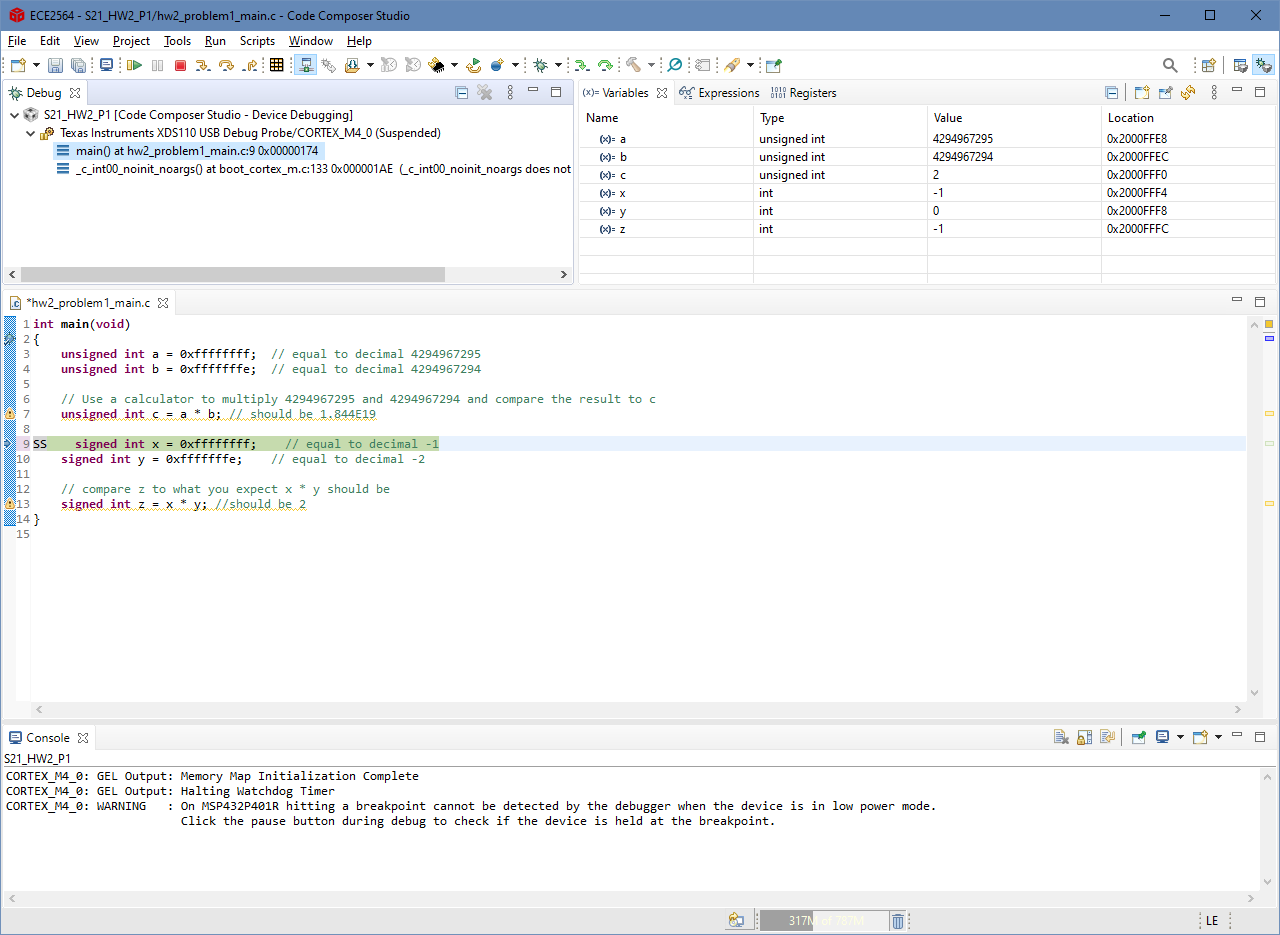
\includegraphics[width = .9\textwidth]{1e.png}
            
            There is an error with the calculation, what likely happened was due to overflow since both numbers were incredibly large and close to the positive cap for unsigned numbers which resulted in a very low outcome to the answer.    
        \end{center}
        \newpage
        \item Post a screenshot of the debug screen on the CCS client:
        \begin{center}
            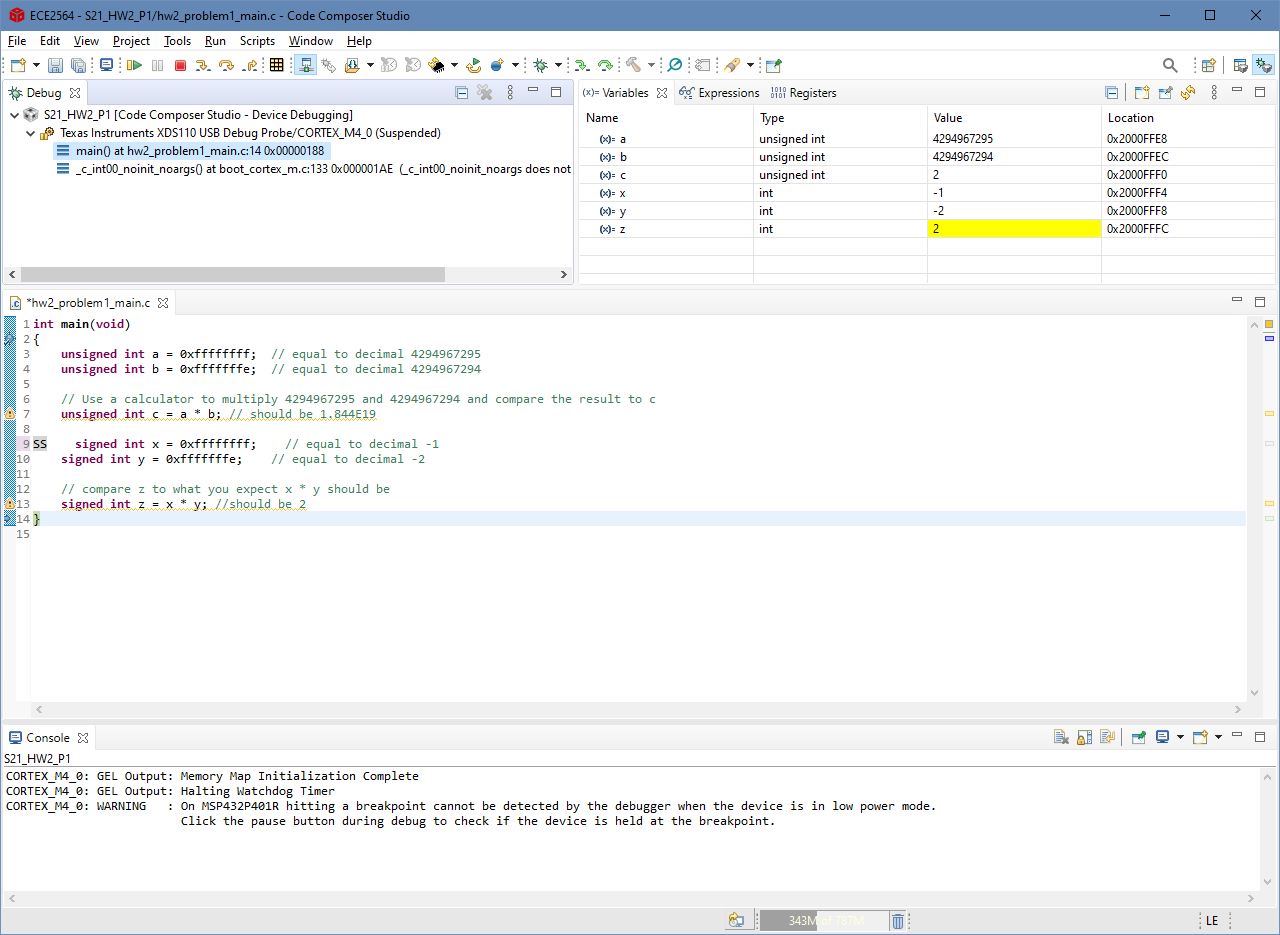
\includegraphics[width = .9\textwidth]{1f.png}
            
            I believe while the output is correct the way it got there is incorrect.
        \end{center}
        \newpage
        \item Fix the code show that the variables are fixed in the debug menu and post the code.
        \begin{center}
            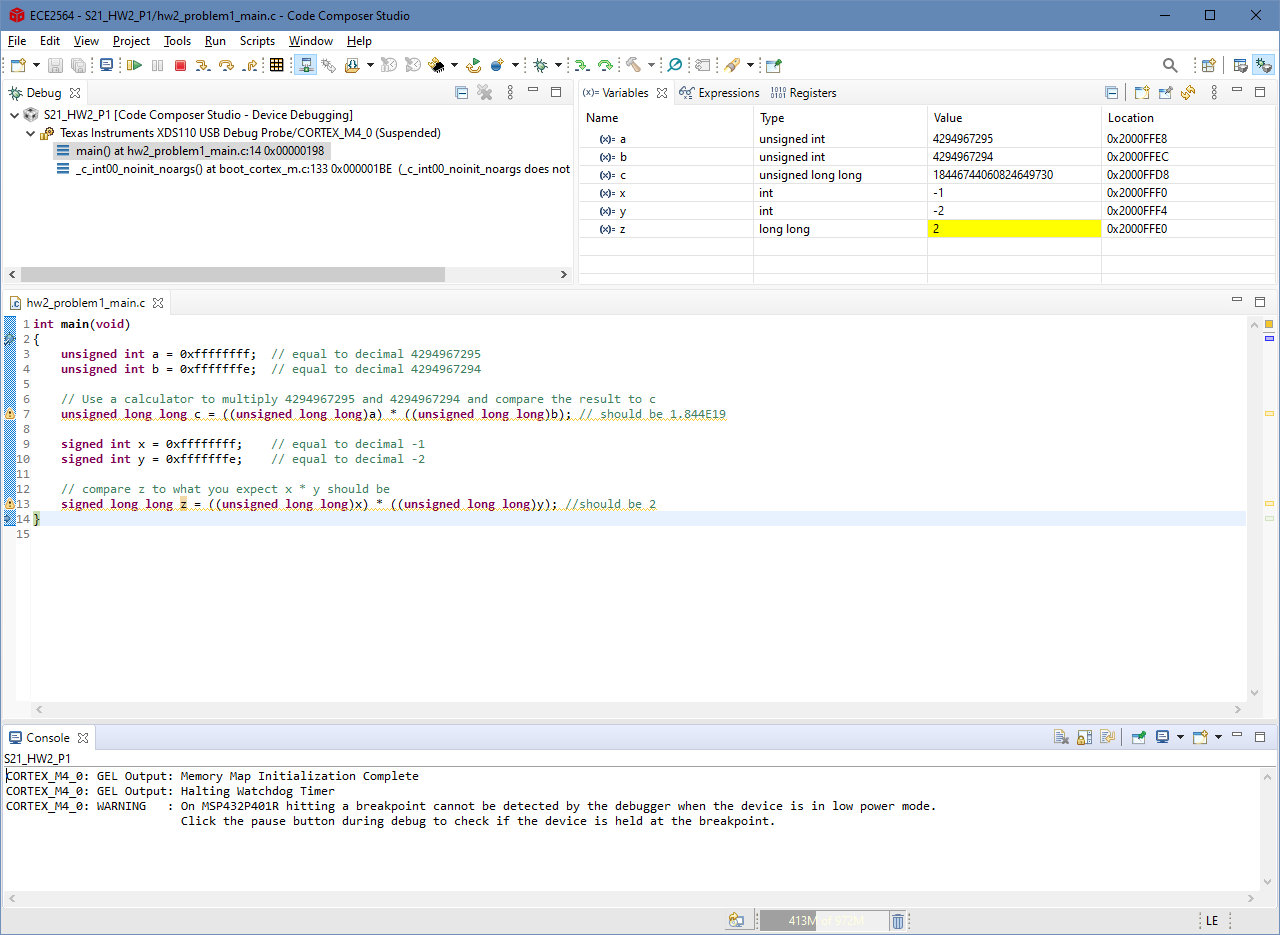
\includegraphics[width = .9\textwidth]{1g.png}
            
            This version has the correct outputs for both computations, the code is below:
        \end{center}
        \lstset{language=C}
        \lstset{frame=lines}
        \lstset{label={lst:code_direct}}
        \lstset{basicstyle=\footnotesize}
        \begin{lstlisting}
int main(void){
        unsigned int a = 0xffffffff;  // equal to decimal 4294967295
        unsigned int b = 0xfffffffe;  // equal to decimal 4294967294
    
        unsigned long long c = ((unsigned long long)a) * ((unsigned long long)b); 
    
        signed int x = 0xffffffff;    // equal to decimal -1
        signed int y = 0xfffffffe;    // equal to decimal -2
    
        // compare z to what you expect x * y should be
        signed long long z = ((unsigned long long)x) * ((unsigned long long)y); 
    }
        \end{lstlisting}
    \end{enumerate}
    \newpage
    \item (15 points) In this problem, we will practice debugging using CCS with an array example. The goal of this project is to copy an array into another one with a reversed order.
    \begin{enumerate}
        \addtocounter{enumii}{3}
        \item Show a screen capture of both arrays open in the variable menu:
        
        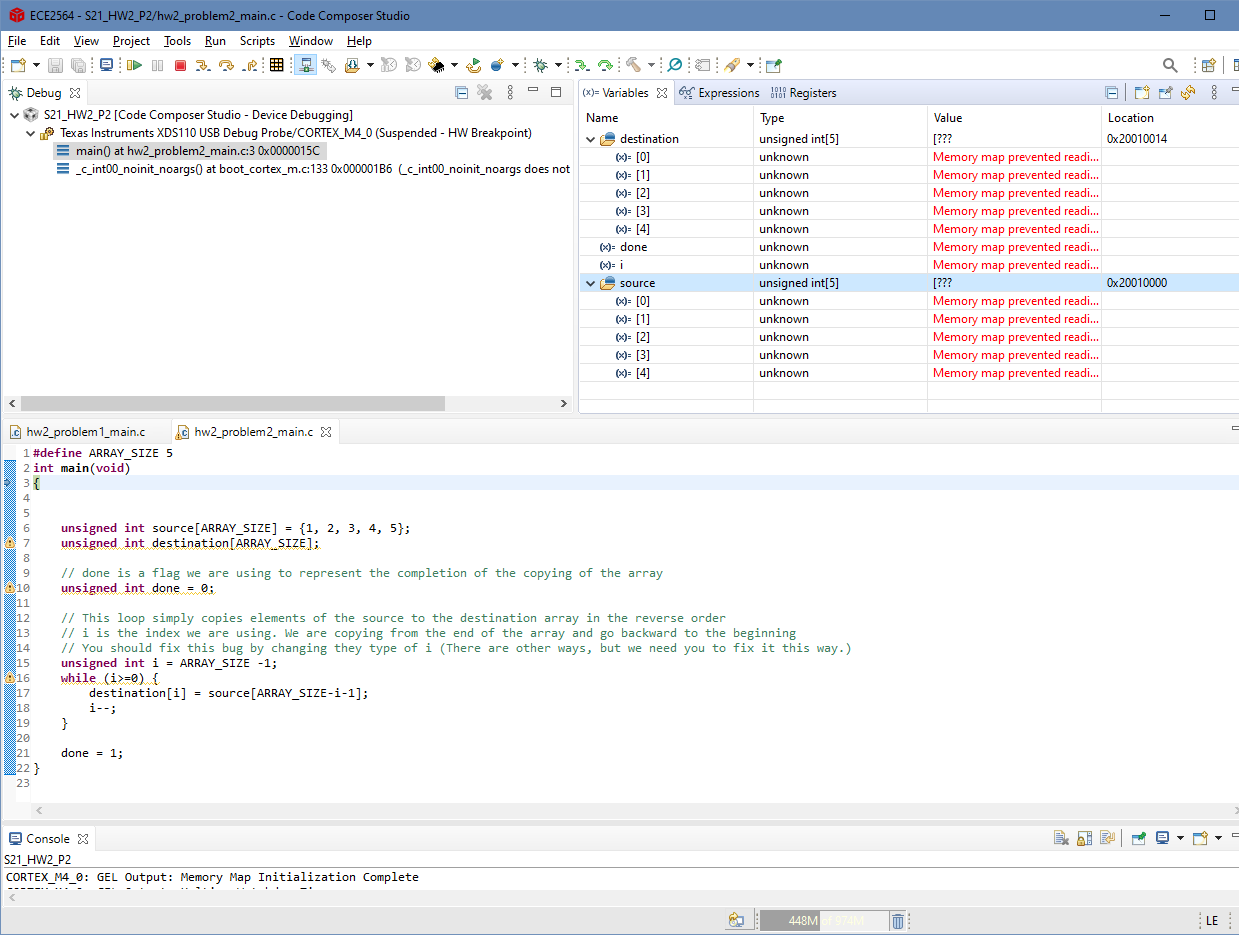
\includegraphics[width = .9\textwidth]{2d.png}
        \newpage
        \item Show a screen capture of what happens when several steps have passed:
        
        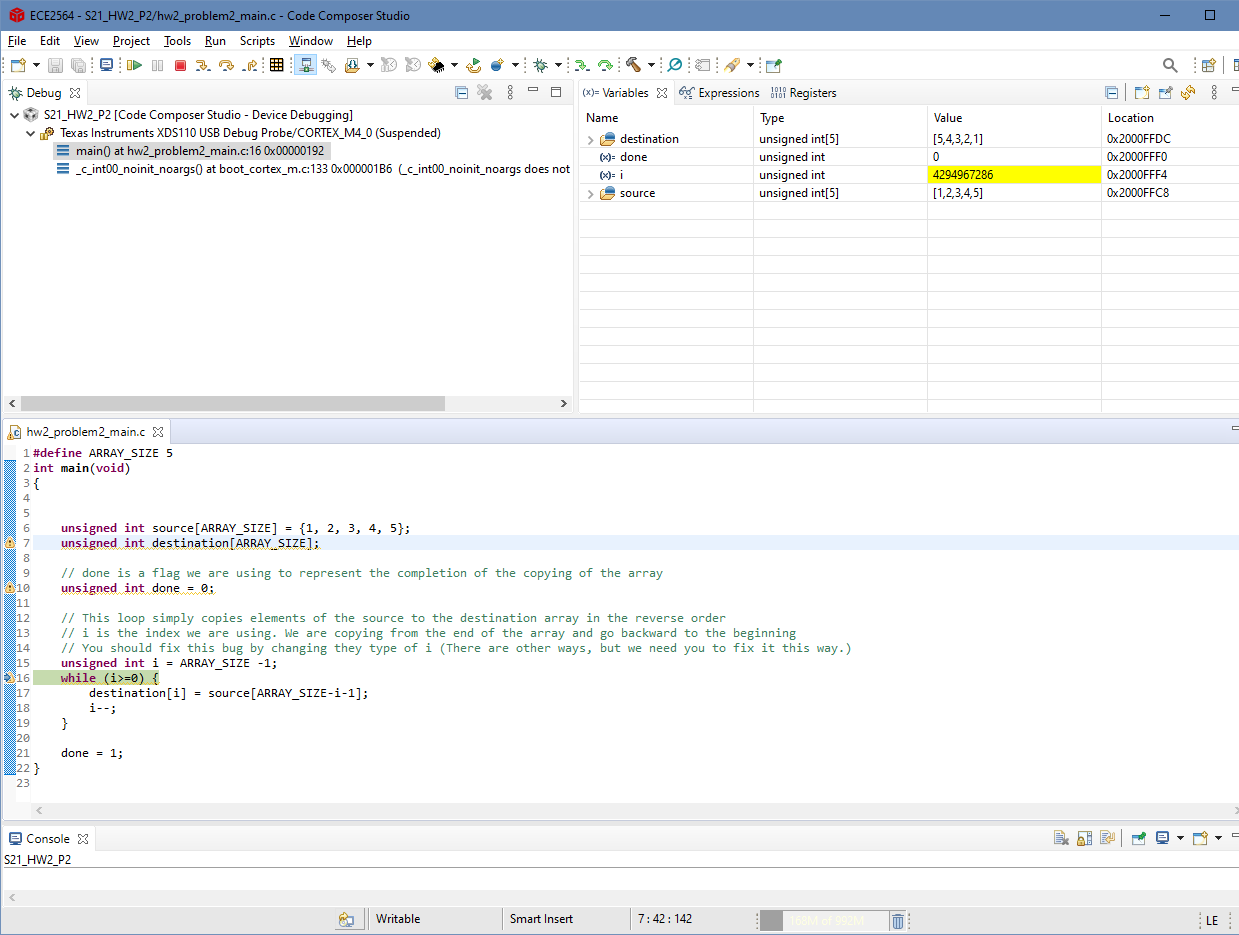
\includegraphics[width = .9\textwidth]{2e.png}
        \newpage
        \item Show a screen capture of the solution:
        
        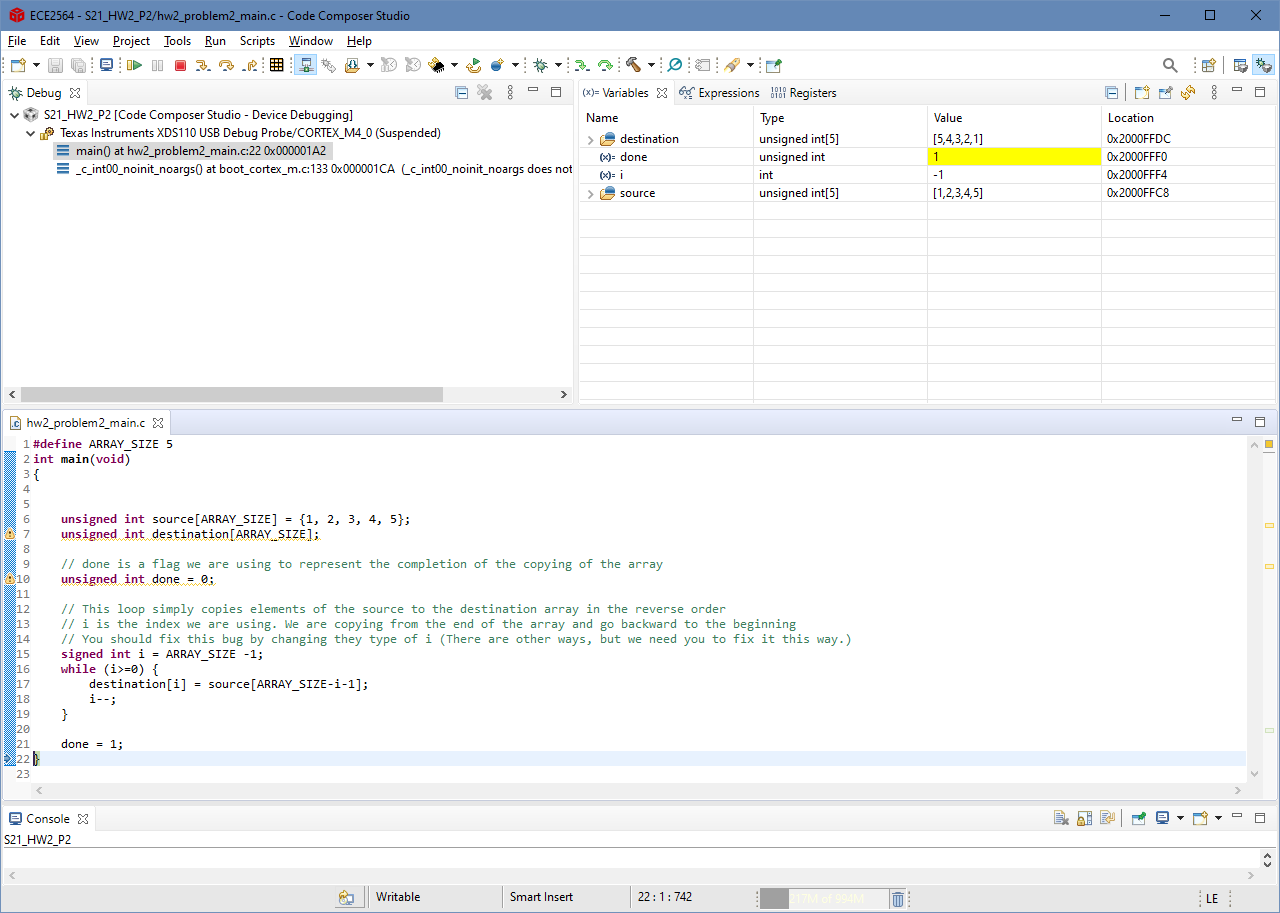
\includegraphics[width = .9\textwidth]{2f.png}
        \begin{center}
            The reason why the loop was not exiting was due to the declaration of the i variable, since it was declared as a unsigned integer, when the variable was decremented past the point of zero, instead of going into the negatives it jumped straight to the highest number in the number line. This is a problem because the way the while loop was meant to exit was by seeing if the variable i was less than zero, and since it jumped to $2^{32}$ this would take a very long time, and when it eventually did get back to zero it would just restart the process. So the solution was to make it a signed integer instead of an unsigned so that it would properly go into the negatives and cause the loop to exit.
        \end{center}
    \end{enumerate}
    \newpage
    \item (60 points) In this problem, we will learn about strings and ASCII code and write a small function. 
    \begin{enumerate}
        \addtocounter{enumii}{2}
        \item Debug until line 41 and screen capture with variables window showing
        \begin{center}
            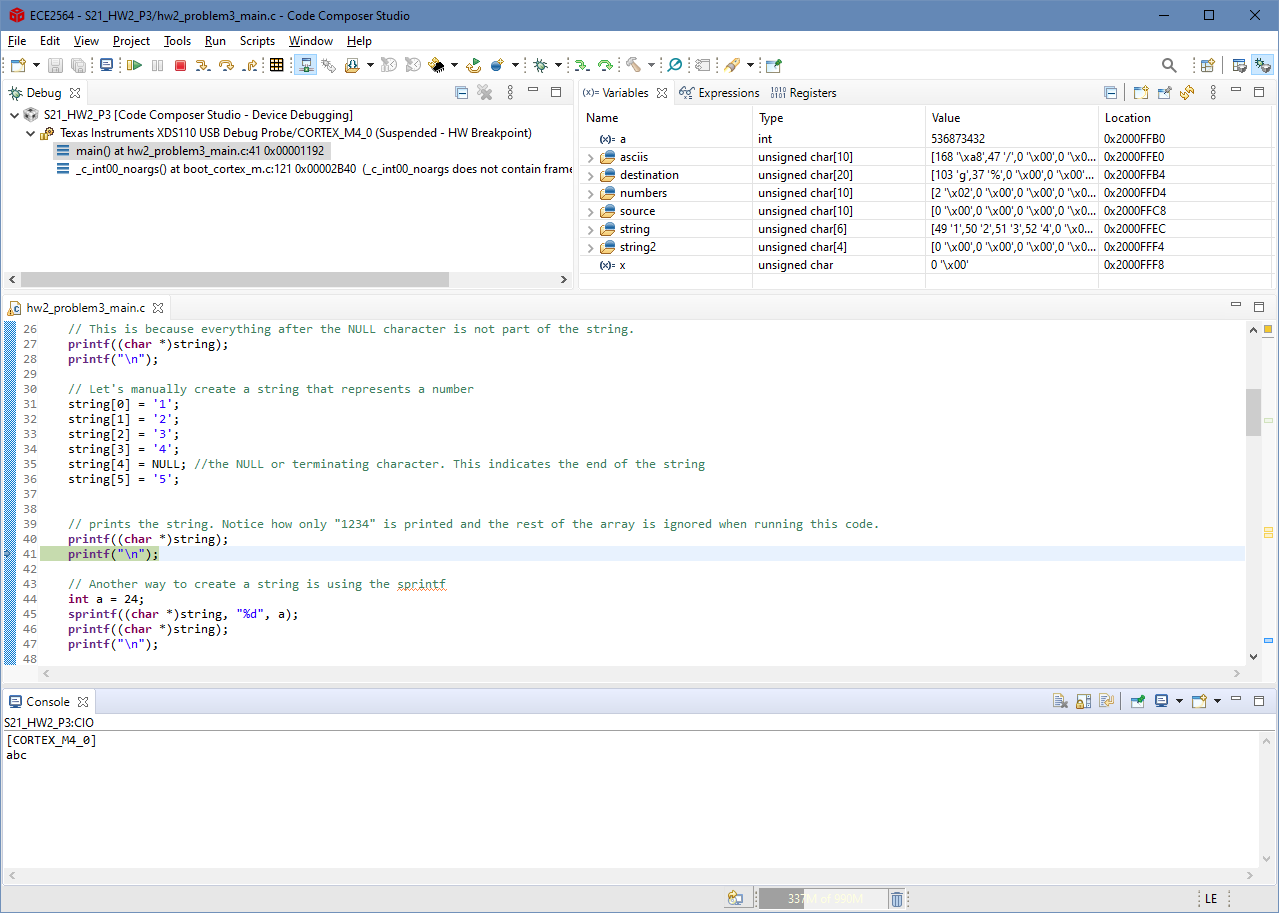
\includegraphics[width = .9\textwidth]{3c.png}
            
            If the string[3] = NULL was true then the output of the program would end up being 123 instead of 1234 this is because the string is getting terminated earlier than usually compared to when the NULL character was at string[4].
        \end{center}
        \addtocounter{enumii}{2}
        \item What is the value of x? What is the content of string2 array?
        \begin{center}
            The value of x is 6 and string2 is currently empty as it has not yet passed the sprintf function.
        \end{center}
        \item
        \begin{center}
            The new value of x when one more step happens becomes zero, I could guess that this has something to do with the way that the sprintf function inserts the NULL terminating character into the string but that could very easily be wrong.
        \end{center}
        \addtocounter{enumii}{1}
        \newpage
        \item What is printed for string2 in the console? Is it different from what you wish it to be? Take a screenshot and attach it to your solution. Explain in a sentence or two what is wrong with string2.
        \begin{center}
            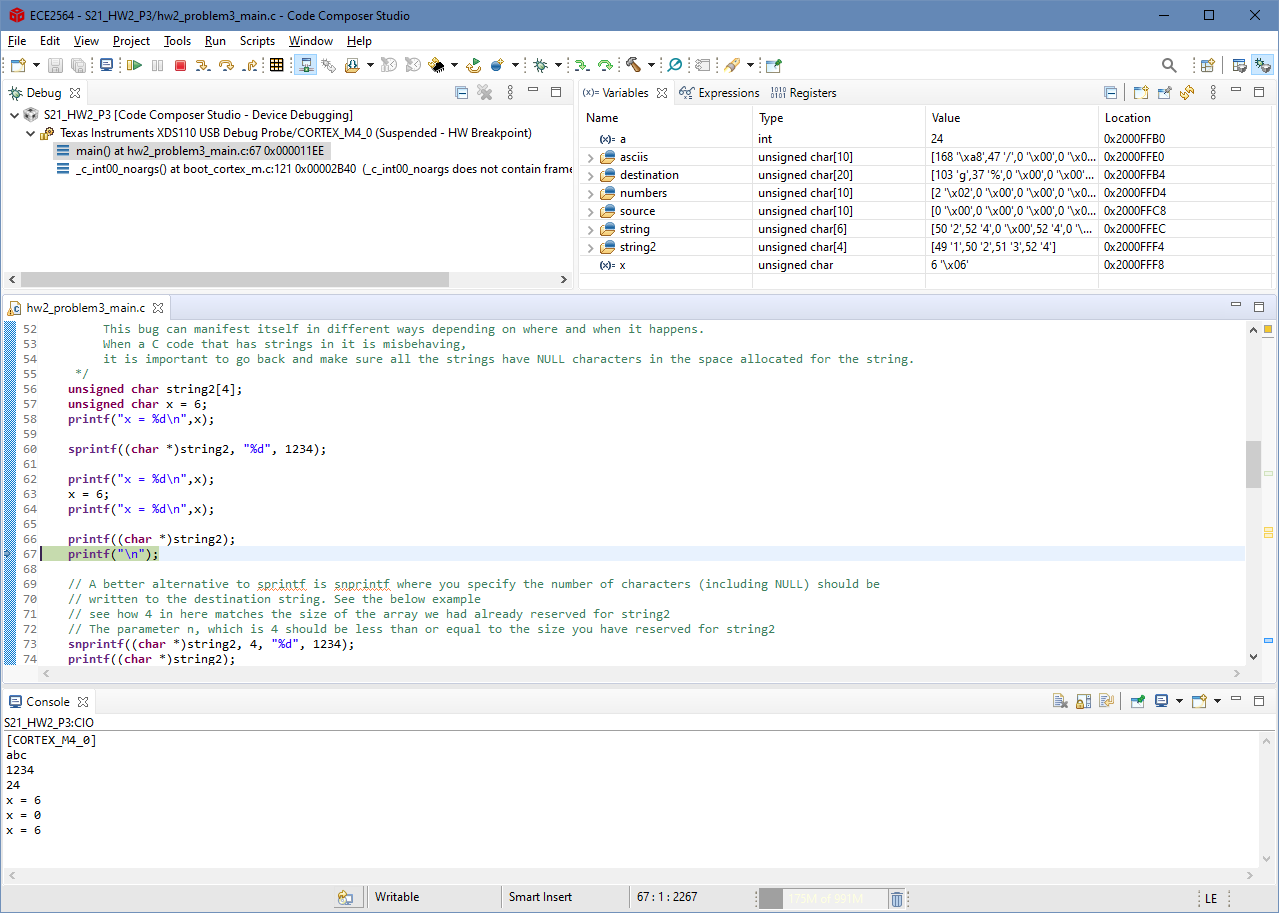
\includegraphics[width = .9\textwidth]{3i.png}
        
            x = 6 is printed as string two, which is not what we wanted to print originally. What the original string was meant to be was "1234" which has seems to have disappeared somewhere in the process.
        \end{center}
        \addtocounter{enumii}{1}
        \newpage
        \item Did  snprintf  corrupt  x  like  sprint  did?  Is  string2 representing what you were hoping ‘1234’? Explain your observation.
        \begin{center}
            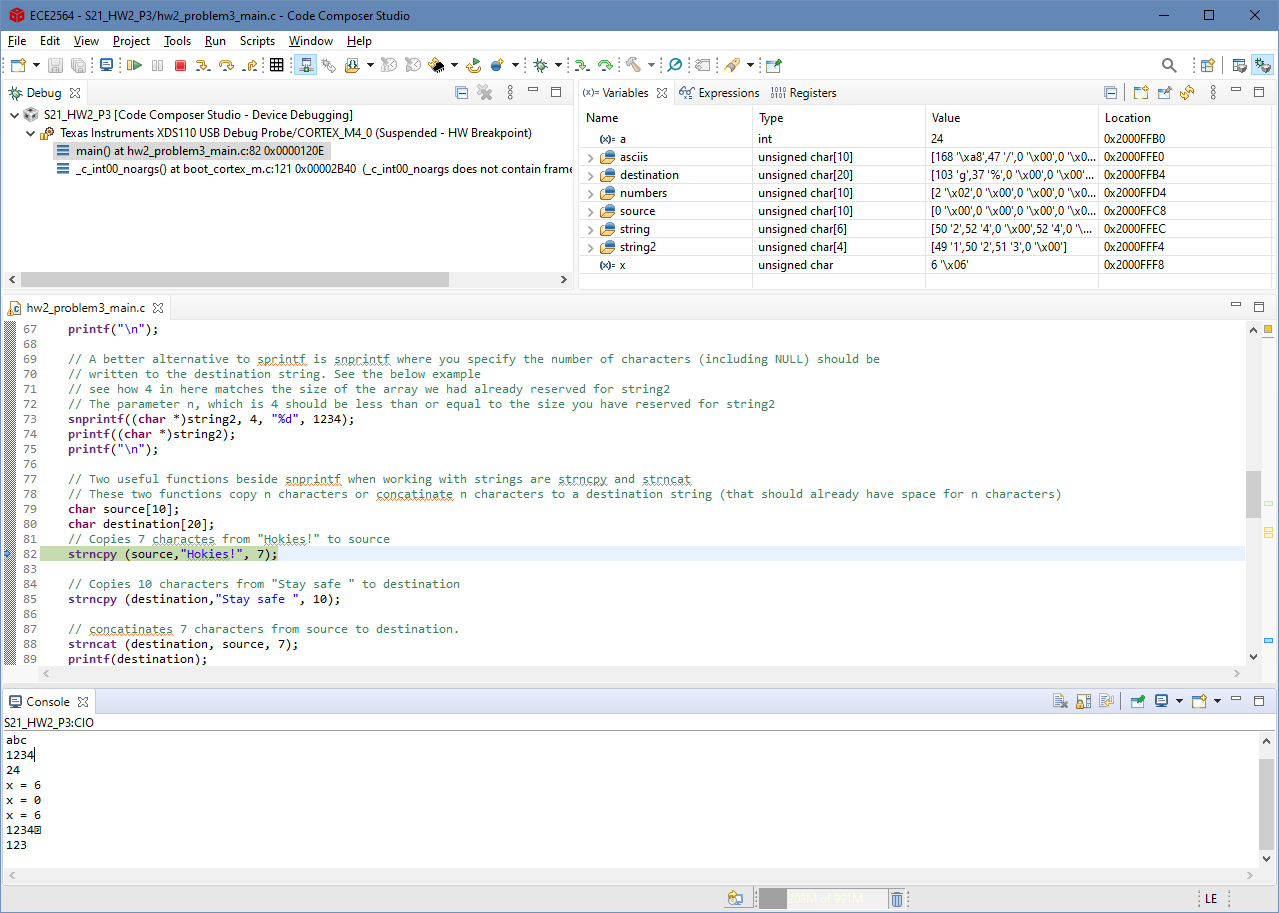
\includegraphics[width = .9\textwidth]{3k.png}
            
            It did not corrupt but only printed three out of the four needed characters, this is because in the snprintf declaration only four characters were listed, but there needs to be five since one of those characters is reserved for the NULL space.
        \end{center}
        \item Try to fix the error you observed earlier where x was corrupted and string2 was not as we expected. Copy paste your fix to your document solution (this file?). Explain how this fixes the problem in a sentence or two.
        \begin{center}
        \lstset{language=C}
        \lstset{frame=lines}
        \lstset{label={lst:code_direct}}
        \lstset{basicstyle=\footnotesize}
        \begin{lstlisting}
        unsigned char string2[4];
        unsigned char x = 6;
        printf("x = %d\n",x);
        printf("x = %d\n",x);
        x = 6;
        printf("x = %d\n",x);
        sprintf((char *)string2, "%d", 1234);
        printf((char *)string2);
        printf("\n");
        \end{lstlisting}
        
        By moving the sprintf function directly above the line where the printing occurs we can avoid the corruption of the data and get the proper output.
        \end{center}
        \newpage
        \item after the the errors are fixed debug until line 77 and see if the output is correct.
        \begin{center}
            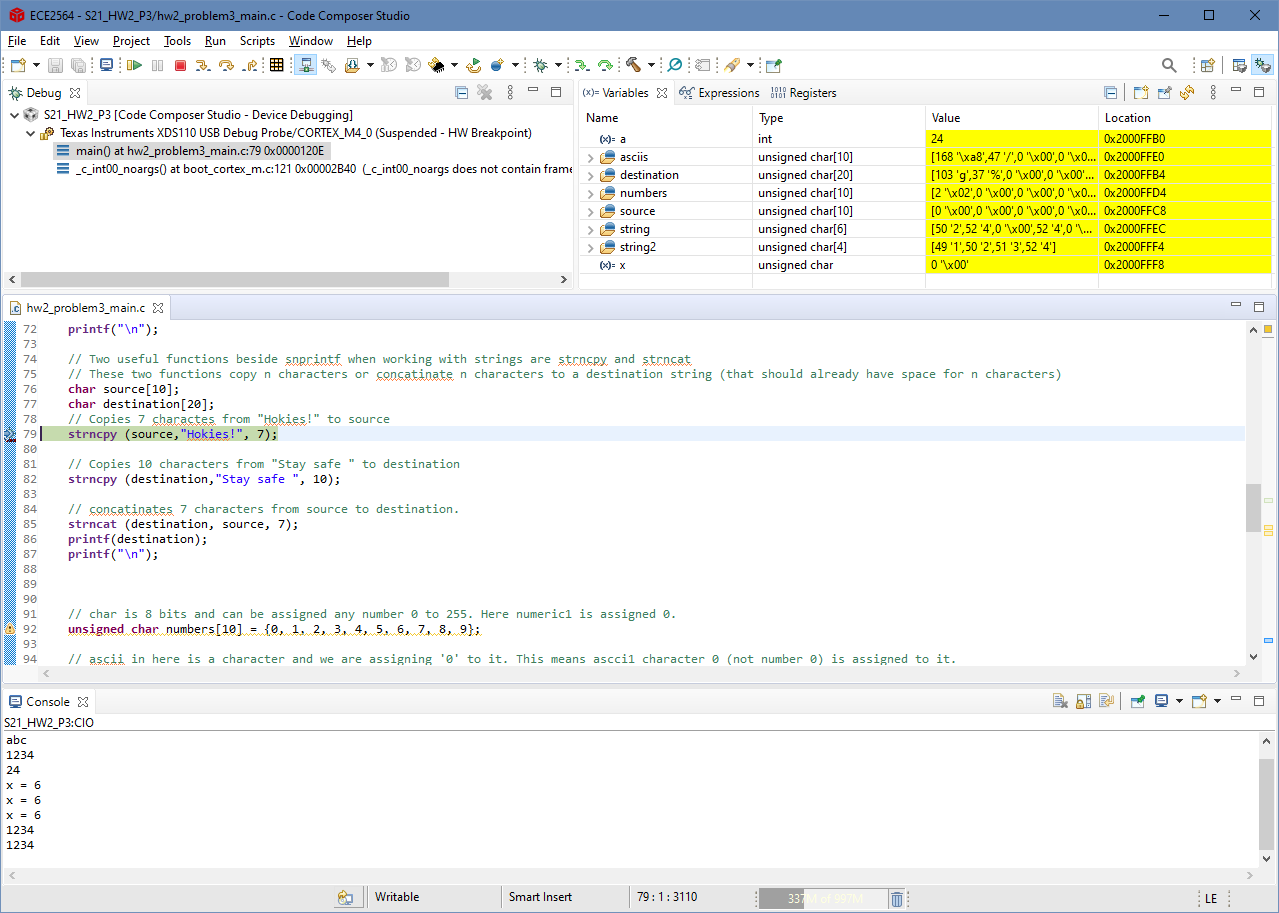
\includegraphics[width = .9\textwidth]{3m.png}
        \end{center}
        \newpage
        \item debug until line 90 and post a screenshot.
        \begin{center}
            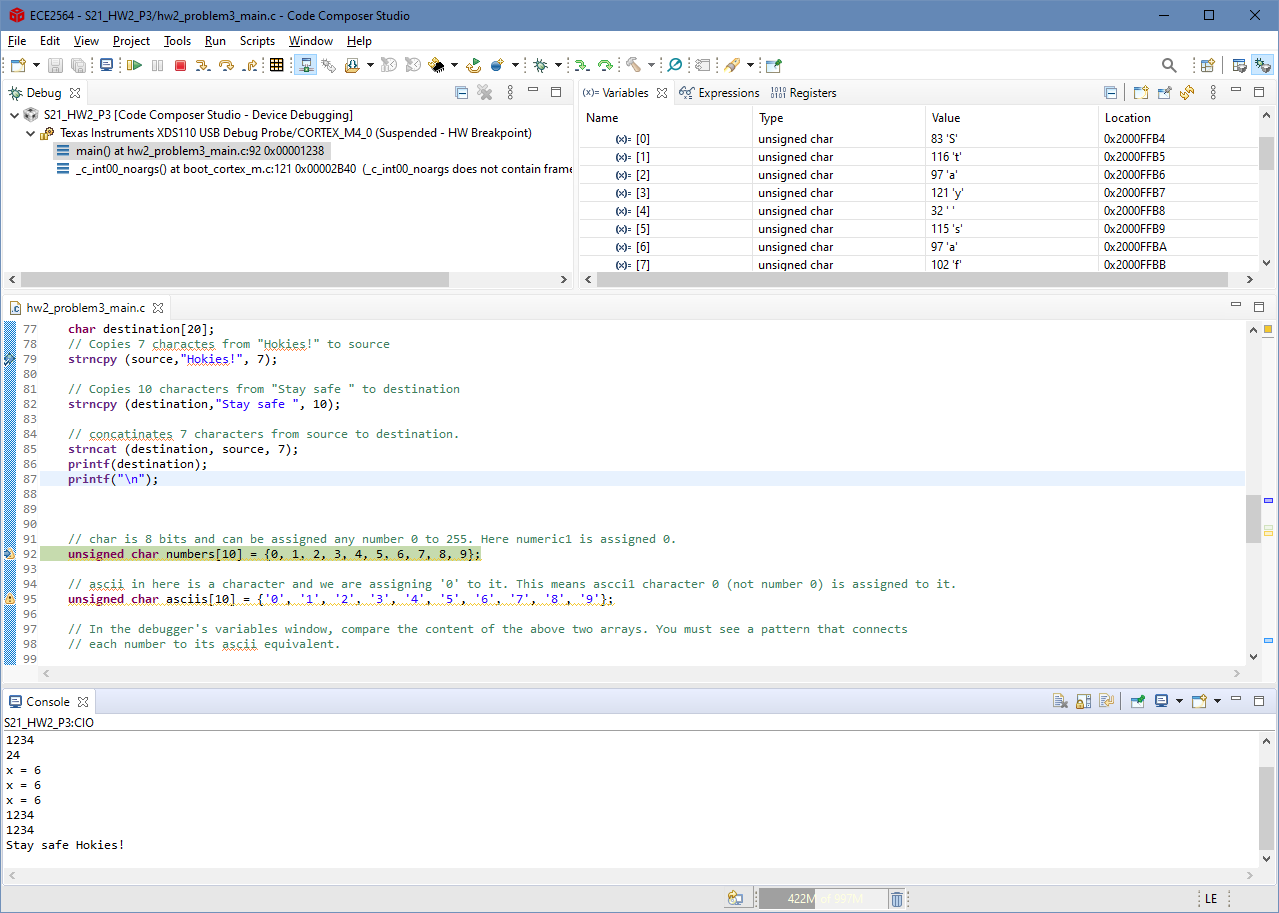
\includegraphics[width = .9\textwidth]{3n.png}
        \end{center}
        \addtocounter{enumii}{6}
        \newpage
        \item Copy and paste the code you have developed for the function in your solution file.
        \lstset{language=C}
        \lstset{frame=lines}
        \lstset{label={lst:code_direct}}
        \lstset{basicstyle=\footnotesize}
        \begin{lstlisting}
void make_time_string(int min, int sec, unsigned char *string) {
    sprintf((char *)string, "%02d:%02d", min, sec);
}
        \end{lstlisting}
    \end{enumerate}
\end{enumerate}

\end{document}
